\section{Dominant-set clustering}\label{ch5} 
We now focus on \textbf{unsupervised learning} problems, i.e. \textbf{clustering}, and in particular we focus on the \textbf{dominant set} approach for solving such problems.

\subsection{Graph-theoretic definition of a cluster}
These notes are based on \cite{pavan2006dominant}.

Data to be clustered are represented as an undirected weighted graph with no self-loops: $G=(V, E, \omega)$, where $V=\{1,\dots,n\}$ is the vertex set, $E\subseteq V\times V$ is the edges set and $w: E\rightarrow \mathbb{R}^*_+$ is the positive weight function. Vertices represent data points, edges neighborhood relationships and edge-weights similarity relations. $G$ is then represented with an adjacency matrix $A$, such that $a_{ij} = \omega(i,j)$. Since there are not self-loops we have that $\omega(i,i) = 0$ (main diagonal equal to $0$). From now on, if not otherwise stated, $A$ will represent such matrix. \\
There is \textbf{not} an \textbf{unique} and well defined \textbf{definition} of \textbf{cluster}, but the available literature agrees in two conditions that a cluster should satisfy:
\begin{itemize}
  \item \textbf{High internal homogeneity}, also named \textit{internal criterion}. It means that all the objects inside a cluster should be highly similar to (or have low distance from) each other;
  \item \textbf{High external inhomogeneity}, also named \textit{external criterion}. It means that objects coming from different clusters have low similarity (or high distance).
\end{itemize}
The idea of these criterion is that \textbf{clusters} are groups of objects which are \textbf{strongly similar} to each other if they belong to the same cluster, otherwise they are \textbf{highly dissimilar}. 

\paragraph{Basic definitions.}

Let $S\subseteq V$ be a nonempty subset of vertices and $i \in S$. The \textbf{average weighted degree} of $i$ w.r.t. $S$ is defined as:
\begin{equation}
  \text{awdeg}_S(i)=\frac{1}{|S|}\sum_{j\in S}a_{ij}
\end{equation}
, i.e. it represents the \textbf{average similarity} between entity $i$ and the rest of the entities in $S$. It can be observed that $\text{awdeg}_{\{i\}}(i) = 0$  $\forall i \in V$, since we have no self-loops.\\

\image{img/awdeg.png}{Visual representstion of $\phi$}{0.25}

We now introduce a new quantity $\phi$ such that if $j \notin S$:
\begin{equation}
  \phi_S(i, j)=a_{ij}-\text{awdeg}_S(i)
\end{equation}

Intuitively, $\phi_S(i, j)$ measures the \textbf{relative similarity} between $i$ and $j$ with respect to the \textbf{average similarity} between $i$ and its neighbors in $S$. This measures can be either positive or negative.

Let $S\subseteq V$ be a nonempty subset of vertices and $i \in S$. The \textbf{weight} of $i$ w.r.t. $S$ is:
\begin{equation}
  w_S(i)= \begin{cases}
      1 & \text{if } |S| = 1 \text{  (singleton)}\\
      \sum\limits_{j\in S\setminus \{i\}}\phi_{S\setminus \{i\}}(j, i)w_{S\setminus \{i\}}(j) & \text{otherwise}
  \end{cases}
\end{equation}

Furthermore, the \textbf{total weight} of $S$ is defined to be $W(S)=\sum_{i\in S}w_S(i)$.
\image{img/ws.png}{Weight of i w.r.t. the elements in S.}{0.18}
Note that $w_{\{i, j\}}(i)=w_{\{i, j\}}(j)=a_{ij}$ $\forall i, j \in V \land i\neq j$. Then, $w_S(i)$ is computed simply as a function of the weights on the edges of the sub-graph induced by $S$.

Intuitively, $w_S(i)$ gives a measure of the \textbf{similarity} between $i$ and $S\setminus \{i\}$ with respect to the \textbf{overall similarity} among the vertices of $S\setminus \{i\}$. In other words, it represents \textbf{how similar (important)} $i$ is \textbf{with respect to the entities} in $S$. An important property of this definition is that it induces a sort of \textbf{natural ranking} among the \textbf{vertices} of the graph. 

\begin{figure}[h!]
		\centering
        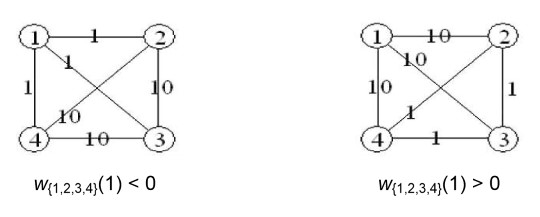
\includegraphics[scale = 1.0]{img/total weight rxample.jpg}
		\label{mi}
        \caption{Examples of total weight}
\end{figure}

As we can see, in the first example we should not add node 1 to the cluster \{2,3,4\}, since it has a low similarity compared with the other nodes (as it can be seen from the value of the total weight), while in the second case we would add node 1 in order to obtain a larger and more coherent cluster.

\paragraph{Dominant set.} A nonempty subset of vertices $S\subset V$ such that $W(T)>0$ for any nonempty $T \subseteq S$, is said to be a \textbf{dominant set} if:
\begin{itemize}
  \item $w_S(i) > 0$, $\forall i \in S \qquad$ (\textit{internal homogeneity})
  \item $w_{S \cup \{i\}}(i) < 0$, $\forall i \notin S \qquad$ (\textit{external homogeneity})
\end{itemize}
These conditions correspond to cluster properties (\textbf{internal homogeneity} and \textbf{external in-homogeneity}). Informally we can say that the \textbf{first condition} requires that \textbf{all the nodes} in the clusters are \textbf{important} for it. The \textbf{second} one assumes that if we consider a \textbf{new point} in the cluster, the \textbf{cluster cohesiveness will be lower}, meaning that the current cluster should be already maximal.\\
By definition, dominant sets are expected to capture \textbf{compact structure}s. Moreover, this definition is equivalent to the one of maximal clique problem when applied to unweighted graphs.

\image{img/dominant_def}{The set of vertices \{1,2,3\} is dominant.}{0.2}

\subsection{Connections of dominant sets}
Dominant sets have intriguing connections with:

\begin{itemize}
    \item \textbf{Game theory}, and concepts like Nash equilibria;
    \item \textbf{Optimization theory}, in particular they are local maximizers of (continuous) quadratic problems;
    \item \textbf{Graph theory} and \textbf{maximal cliques};
    \item \textbf{Dynamical systems theory}.
\end{itemize}

\subsubsection{Optimization theory}
\textbf{Clusters} are commonly represented as $n$-dimensional \textbf{vectors} expressing the participation of each node to a cluster. Large numbers denote a strong participation, while zero values no participation. The \textbf{cohesiveness} of a cluster can be computed using:
\begin{equation}
f(x)=x^\top Ax
\end{equation}
where $A$ is the \textbf{symmetric} real-valued matrix with null diagonal. \textbf{Clustering} can now be formulated as the problem of \textbf{finding the vector} $x$ that \textbf{maximizes} $f$. The objective function has to be \textbf{normalized}. For this aim simplex constraints are imposed. This yields the following \textbf{standard quadratic optimization problem} whose \textbf{local solution} corresponds to a \textbf{maximally cohesive cluster}:
\begin{equation}\label{SPQ}
\begin{array}{lcl}
\text{max} & x^TAx \\
\text{s.t.} & x \in \Delta
\end{array}
\end{equation}
where
\begin{equation}
\Delta=\{x\in\mathbb{R}^n:x\geq 0 \land x^\top x = 1\}
\end{equation}
is the \textbf{standard simplex} of $\mathbb{R}^n$.\\

\image{img/standardSimplex.png}{Standard simplex on $\mathbb{R}^3$.}{0.35}

In conclusion \textbf{dominant sets} can be put in \textbf{one-to-one correspondence} (modulo a technical condition) with \textbf{strict local maximizers} of a \textbf{quadratic function over the simplex}, i.e., given a dominant set we can build $x \in \Delta$, which is a strict local maximum of $x^TAx$. 

\subsubsection{Graph theory and maximal cliques}
Suppose we have a \textbf{binary similarity matrix} and an unweighted undirected graph $G = (V,E)$, then:

\begin{itemize}
    \item A \textbf{clique} is a subset of mutually adjacent vertices;
    \item A \textbf{maximal clique} is a clique that is not contained in a larger one;
\end{itemize}

It was proved that \textbf{dominant sets} are in \textbf{one-to-one correspondence} to \textbf{maximal cliques} of $G$. 

\subsection{Finding dominant sets}
One of the major \textbf{advantages} of using \textbf{dominant sets} is that the procedure that allows to find them can be written with few lines of code. There are several dominant set clustering approaches:
\begin{itemize}
	\item To get a \textbf{single} dominant set cluster use \textbf{replicator dynamics};
	\item To get a \textbf{partition} use a simple \textit{peel-off} strategy: iteratively find a dominant set and remove it from the graph, until all vertices have been clustered;
	\item To get \textbf{overlapping clusters}, enumerate dominant sets. 
\end{itemize}

The \textbf{replicator dynamics} (RD) are \textbf{deterministic game dynamics} that have been developed in evolutionary game theory, and allow to find DS's. The computation is the following:
$$
x_i(t+1) = x_i(t)\frac{A(x(t))_i}{x(t)^TAx(t)}
$$

\image{img/rep_dynamics}{MATLAB implementation of discrete-time replicator dynamics}{0.4}

As we can see, the algorithm generates a sequence of points in the standard simplex $\Delta$, and if $A$ is a symmetric matrix, it converges to a strict local maximum.

The components of the \textbf{converged vector} give us a measure of the \textbf{participation} of the corresponding vertices in the cluster, while the \textbf{value} of the \textbf{objective function} measures the \textbf{cohesiveness} of the cluster.

\subsection{Properties}
\begin{itemize}
	\item \textbf{Well separation between structure and noise.} In such situations it is often more important to cluster a small subset of the data very well, rather than optimizing a clustering criterion over all the data points, particularly in application scenarios where a large amount of noisy data is encountered;
	
	\item \textbf{Overlapping clustering}. In some cases we can have that two distinct clusters share some points, but partitional approaches impose that each element cannot be long to more than one cluster;
	
	\item Dominant sets can be found by mining \textbf{local solutions}, so it is not necessary to look for global solutions;
	
	\item Performs very well in presence of \textbf{noise} and \textbf{outliers};
		
	\item Makes \textbf{no assumptions} on the \textbf{structure} of the \textbf{affinity matrix}, being it able to work with asymmetric and even negative similarity functions;
	
	\item Does \textbf{not} require a \textbf{priori knowledge} on the \textbf{number of clusters} (since it extracts them sequentially).
	
	\item Leaves \textbf{clutter} elements \textbf{unassigned} (useful, e.g., in figure/ground separation or one-class clustering problems);
	
	\item Generalizes naturally to \textbf{hypergraph clustering problems};

        \item It allows to rank cluster's elements according to their \textbf{centrality}.
\end{itemize}

\subsection{Image segmentation}
An image is represented as an edge-weighted undirected graph, where \textbf{vertices} correspond to \textbf{individuals pixels} and edge-weights reflect the \textbf{similarity} between pairs of vertices. The \textbf{clustering} problem consists on extracting \textbf{dominant sets} from an input image, below is proposed the pseudo-code version of the solution with dominant sets:

\image{img/dominantSetAlg.png}{Pseudo-code for image segmentation.}{0.5}
Remember that to find a single dominant set we used replicator dynamics.

\subsection{Conversational groups detection}
\footnote{This section is based on \cite{vascon2016detecting}.}

We now focus on the problem of \textbf{conversational groups detection}. Formally, a conversational group, also called \textbf{F-formations}, exists when \textit{"two or more individuals in close proximity orient their bodies in such a way that each of them has an easy, direct and equal access to every other participant's transactional segment"}. Picture \ref{f-formations} provides an example of F-formations.

\begin{figure}[h!]
    \centering
    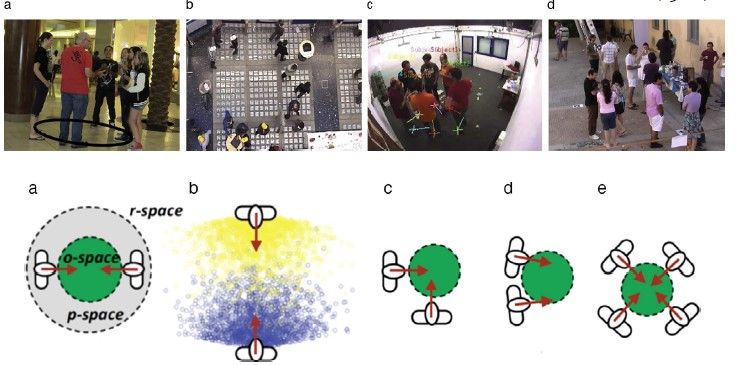
\includegraphics[scale = 1.5]{img/f-formations.jpg}
    \label{f-formations}
    \caption{Example of F-formations}
\end{figure}


Picture \ref{groups detection arch} shows the architecture for solving this problem.

\begin{figure}[h!]
    \centering
    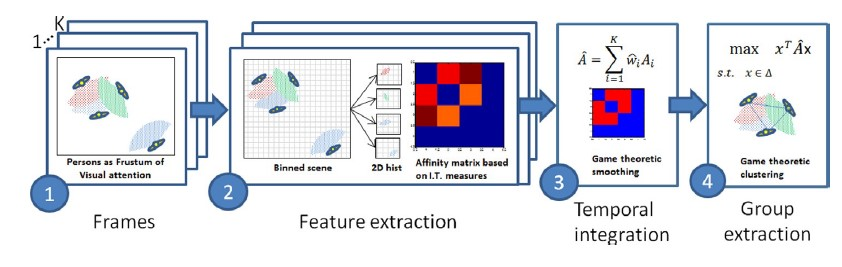
\includegraphics[scale = 1.5]{img/groups detection.jpg}
    \label{groups detection arch}
    \caption{Architecture for solving the groups detection problem}
\end{figure}

As we can see, the architecture is composed of 4 phases:

\begin{enumerate}
    \item The first takes as input an image, and it is responsible for creating the \textbf{frames}. In the frames the \textbf{persons} are represented with the so-called \textbf{frustrum of visual attention}: each \textbf{person} in the scene is described by his/her \textbf{position} $(x,y)$ and by the \textbf{head rotation} $\theta$. The \textbf{frustrum} represents the \textbf{area} in which a person can sustain a conversation, and it is defined by an \textbf{aperture} and by a \textbf{length}. The intuition is that the \textbf{more} two frustra \textbf{overlap}, the \textbf{higher} the \textbf{probability} of two people to \textbf{interact};
    \item The second phase implements the \textbf{feature extraction} from the frame: the idea is to create a \textbf{graph} in which the \textbf{nodes} are the \textbf{persons}, while the \textbf{edges} represents the \textbf{probability} of interaction between them, calculated as the overlap of the corresponding frustra;
    \item \textbf{Temporal integration};
    \item \textbf{Group extraction}, by using the DS approach. In this case, DS allows to execute the extraction without knowing the number of clusters in advance, and to deal very well with the outliers.
\end{enumerate}

More specifically, this model was executed by providing different ways of computing the overlap between the frustra (e.g. K-L divergence, Jaccard etc..), but in all the cases the algorithm performed better than Spectral Clustering (executed providing the correct number of clusters in advance).

Picture \ref{groups detection res} shows an example of the results: the yellow represents the ground truth, the green represents the result of the model, while red represents the result of another model (HFF).

\begin{figure}[h!]
    \centering
    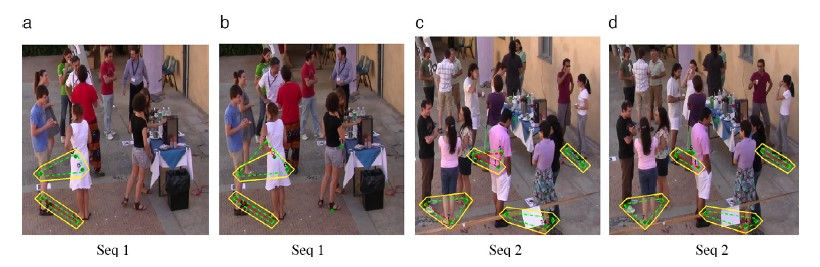
\includegraphics[scale = 1.5]{img/groups detection1.jpg}
    \label{groups detection res}
    \caption{Results of the model}
\end{figure}

\subsection{Constrained image segmentation}
The classical problem of \textbf{image segmentation} consists of \textbf{partitioning} an \textbf{image} into multiple parts or \textbf{regions}, often based on the characteristics of the pixels in the image. Modern \textbf{variations} of the classical (purely bottom-up) approach, involve, e.g., some form of user assistance (\textbf{interactive segmentation}) or ask for the simultaneous segmentation of two or more images (\textbf{co-segmentation}). At an abstract level, all these variants can be thought of as \textbf{“constrained” versions} of the original formulation, whereby the segmentation process is guided by some external source of information. 

In the following sections we describe a model for solving the interactive image segmentation problem.

\subsubsection{Constrained dominant sets}
Before analyzing the model, we briefly introduce the \textbf{constrained DS approach}. The setting is the following: given $S \subseteq V$ and a parameter $\alpha > 0$, we define the following parameterized family of quadratic programs:

\begin{equation}\label{CSD}
\begin{array}{lcl}
\max \qquad f_s^{\alpha} (x) = x^T(A - \alpha \hat{I}_S)x \\
\text{s.t. } \qquad x \in \Delta
\end{array}
\end{equation}

, where $\hat{I}_S$ is the \textbf{diagonal matrix} whose elements are set to 1 in correspondence to the vertices outside $S$, and to 0 otherwise. In this way, the elements of $A$ in the diagonal will be set to $-\alpha$ in correspondence to the vertices outside $S$, and to 0 otherwise, or in other words:

$$
a_{ii} = \begin{cases}
    - \alpha \qquad \text{if } i \not\in S \\
    0 \qquad \text{otherwise}
\end{cases}
$$

An important \textbf{property} of this formulation is that by setting 

$$
\alpha > \lambda_{\text{MAX}} (A_{V - S})
$$

, all the \textbf{local solutions} of \ref{CSD} will have a \textbf{support} containing elements of $S$. Notice that $\lambda_{\text{MAX}} (A_{V - S})$ represents the \textbf{largest} \textbf{eigenvalue} of the sub-matrix of $A$ containing the vertices outside $S$.

In general, solving \ref{CSD} allows to find the \textbf{dominant sets that contain the set of nodes $S \subseteq V$}.


\subsubsection{Interactive image segmentation \footnote{This section is based on \cite{zemene2018dominant}.}}
The \textbf{interactive image segmentation} represents a variant of the classical image segmentation problem. In this case the \textbf{input} of the model is given by an \textbf{image} and some \textbf{annotations}, indicating the region of interest in which performing the segmentation, while the \textbf{output} contains the \textbf{segmentation}. There exit two types of possible annotations:

\begin{itemize}
    \item \textbf{scribbles}, representing the \textbf{foreground} and the \textbf{background};
    \item \textbf{bounding box}, which allows the \textbf{selection} of a portion of the image.
\end{itemize}

Picture \ref{iis1} provides an example of the two possible annotations.

\begin{figure}[h!]
    \centering
    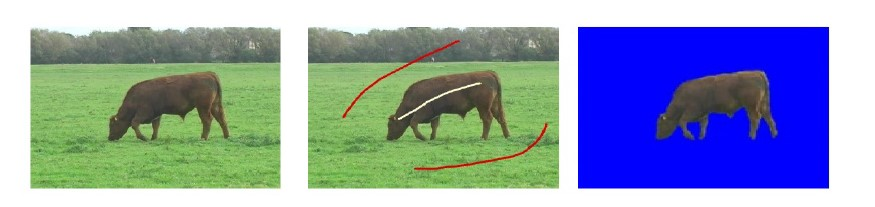
\includegraphics[scale = 1.5]{img/interactive image segmentation.jpg}
    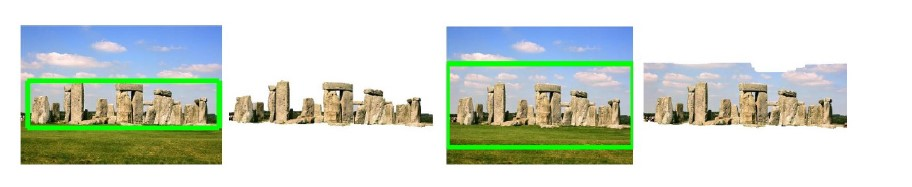
\includegraphics[scale = 1.5]{img/interactive image segmentation1.jpg}
    \label{iis1}
    \caption{Types of annotations}
\end{figure}

Despite being very \textbf{different} from each other, we underline the fact that the \textbf{CDS approach} allows to \textbf{solve} the interactive image segmentation problem with \textbf{both} types, as represented in \ref{iis2}.

 \begin{figure}[h!]
    \centering
    \label{iis2}
    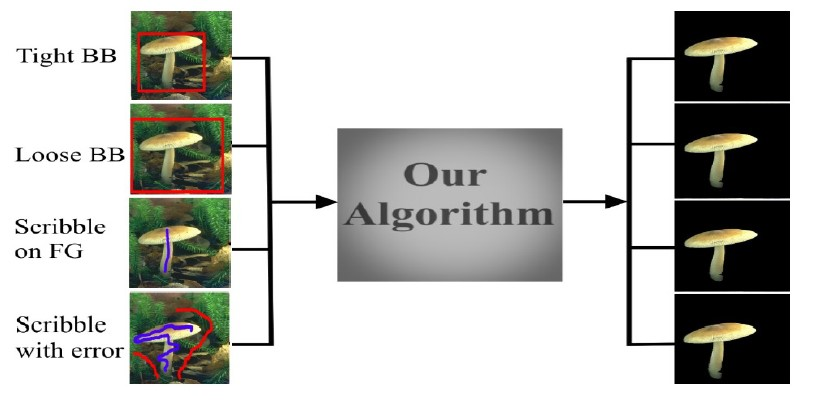
\includegraphics[scale = 1.5]{img/interactive image segmentation2.jpg}
    \caption{Dominant set approach for IIS}
\end{figure}

The \textbf{framework} for solving this problem is showed in \ref{iis3}.

\begin{figure}[h!]
    \centering
    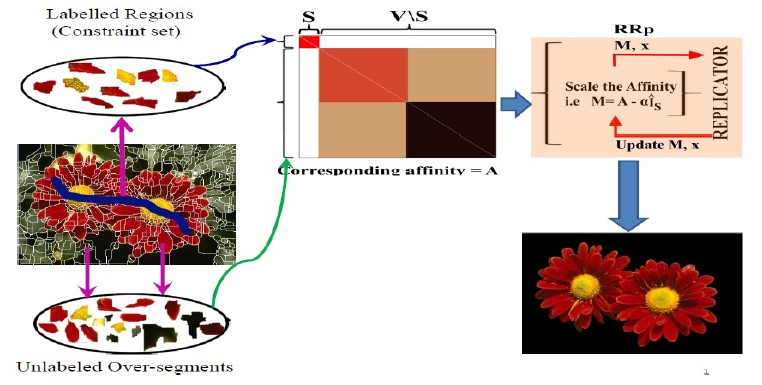
\includegraphics[scale = 1.7]{img/interactive image segmentation3.jpg}
    \label{iis3}
    \caption{Framework}
\end{figure}

The steps are the following:

\begin{enumerate}
    \item We first extract the so-called \textbf{super pixels}, i.e. small contiguous regions of pixels in which the color is homogeneous. This steps allows to reduce the \textbf{dimensionality} of the problem;
    \item Then, the idea is to create a \textbf{graph}, where each of the super pixel is a node. Moreover, we define a partition of this graph: the set $S$, containing the pixels touched by the scribble, and the set $S-V$ containing all the other pixels. We define the corresponding \textbf{affinity matrix};
    \item We run several times the \textbf{replicator dynamics} algorithm, with input $x$ and the scaled matrix $M = A - \alpha \hat{I}_S$, and we get the dominant sets. Let $L$ be number of extracted dominant sets, and say their union is $\text{UDS} = D_1 \cup D_2 \cup .. \cup D_L$, then:

    \begin{itemize}
        \item For scribble-based approach, UDS represents the segmentation result;
        \item For boundary-based approach, its complement V-UDS represents the result. A bounding box can be indeed consider as a square of scribble, so we need to take the inverse of the union, since the union would retrieve the segmentation of the background.
    \end{itemize}
\end{enumerate}

Picture \ref{iis4} shows some results of the model. As we can see, testing both the scribble and the bounding box results in having a segmentation which is highly similar to the ground truth.

\begin{figure}[h!]
    \centering
    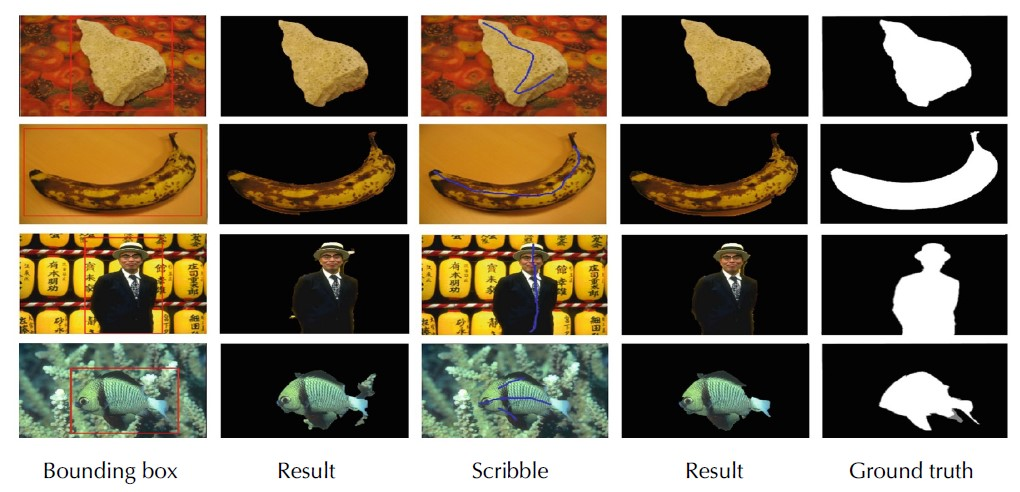
\includegraphics[scale = 1.5]{img/interactive image segmentation4.jpg}
    \label{iis4}
    \caption{Results}
\end{figure}

\subsection{Large-scale image geo-localization}
This section is based on \cite{zemene2018large}.

The \textbf{goal} of this problem is to provide the \textbf{location}, in terms of \textbf{longitude} and \textbf{latitude}, of the location represented in the input image.

\begin{figure}[h!]
    \centering
    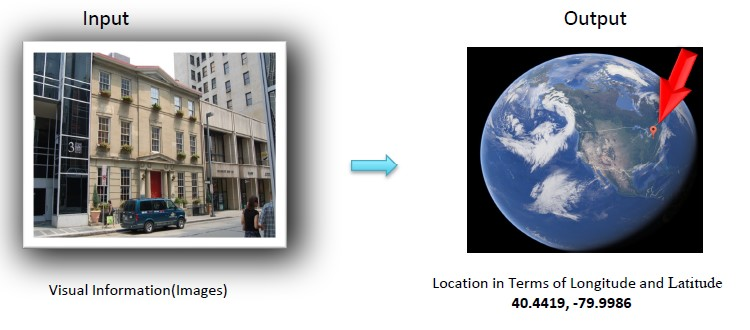
\includegraphics[scale = 1.5]{img/geo1.jpg}
    \label{geo1}
    \caption{Image geo-localization}
\end{figure}

In this case the \textbf{dataset} is composed of \textbf{images} and the relative \textbf{coordinates}, and the goal of the model is to compare the input image with the dataset, and return the coordinates of the closest image. More specifically, for each location the dataset is composed of:

\begin{itemize}
    \item A set of \textbf{4 side views} plus \textbf{1 top view};
    \item A \textbf{label}, corresponding to the \textbf{name} of the location, the \textbf{longitude} and the \textbf{latitude}.
\end{itemize}

An example of the dataset is provided in Picture \ref{geo2}.

\begin{figure}[h!]
    \centering
    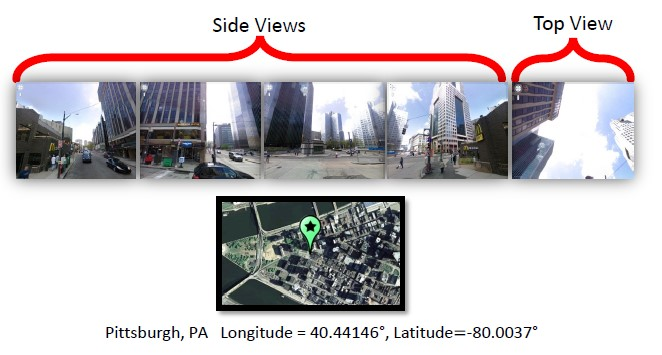
\includegraphics[scale = 1.5]{img/geo2.jpg}
    \label{geo2}
    \caption{Dataset}
\end{figure}

The \textbf{pipeline} for solving this problem is represented in Picture \ref{geo3}.

\begin{figure}[h!]
    \centering
    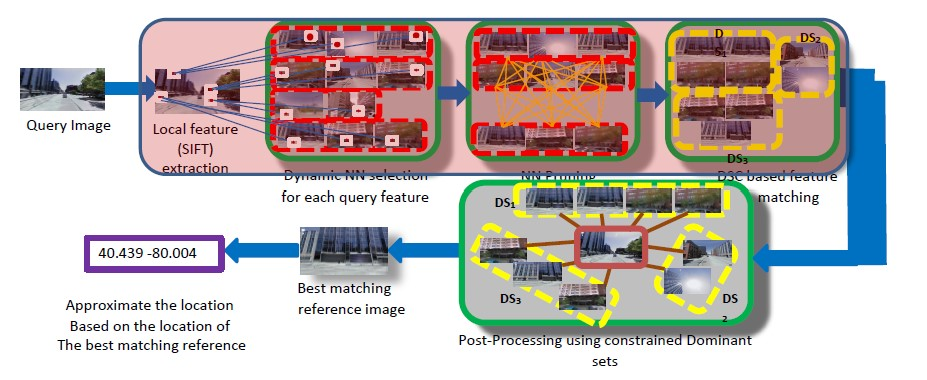
\includegraphics[scale = 1.5]{img/geo3.jpg}
    \label{geo3}
    \caption{Pipeline}
\end{figure}

As we can see:

\begin{enumerate}
    \item The model is provided as \textbf{input} with the \textbf{query image}, i.e. the image for which the location must be localized;
    \item The first operation is the \textbf{local feature (SIFT) extraction}. SIFT features (scale-invariant feature transform) are \textbf{local} and \textbf{based} on the \textbf{appearance} of the object at particular interest points, and are invariant to image scale and rotation. They are also \textbf{robust} to changes in \textbf{illumination}, \textbf{noise}, and \textbf{minor changes} in viewpoint;
    \item Then, the \textbf{dynamic NN selection} occurs: each of the SIFT features is used to get a \textbf{set of the closest images} (and corresponding features) in the dataset;
    \item Then, the \textbf{pruning} phase removes portions of the image corresponding to some outliers;
    \item Then, DS are used for \textbf{clustering} the features, i.e. for matching similar features;
    \item \textbf{Post-processing} using CDS;
    \item Selecting the \textbf{best matching reference image};
    \item Approximate the final \textbf{location} based on the location of the best matching reference image.
\end{enumerate}

The model was trained and tested with the following datasets:

\begin{itemize}
    \item The \textbf{first dataset} is composed of:
    \begin{itemize}
        \item A train set composed of 102k Google street view images from Pittsburgh, PA and Orlando, FL;
        \item A test set composed of 521 GPS-tagged unconstrained images.
    \end{itemize}
    \item The \textbf{second} one is composed of:
    \begin{itemize}
        \item A train set composed of 300k Google street view images from 14 different cities from Europe, North America and Australia;
        \item A test set composed of 500 GPS-tagged unconstrained images.
    \end{itemize}
\end{itemize}

From the \textbf{quantitative results} we notice how the \textbf{CDS} approach followed by the \textbf{post-processing} resulted the best model. Picture \ref{geo4} shows the qualitative results of the model.


\begin{figure}[h!]
    \centering
    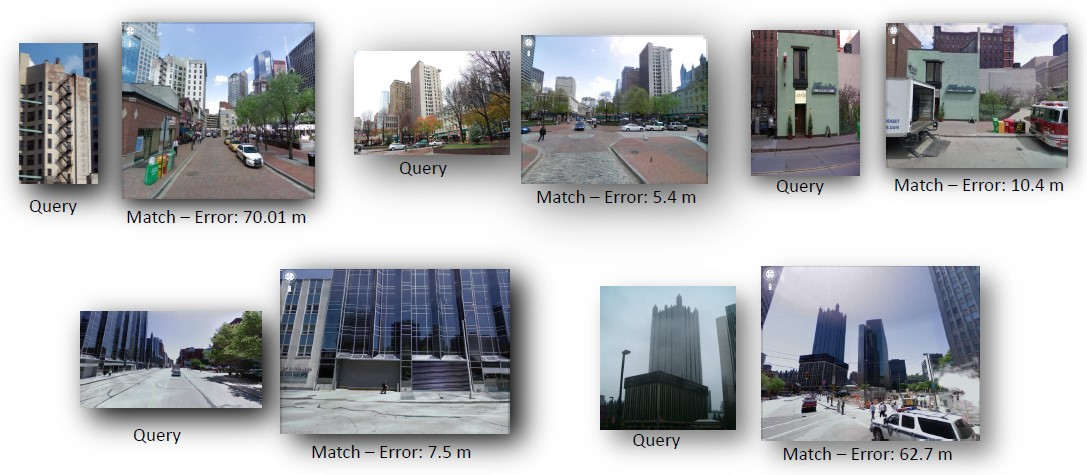
\includegraphics[scale = 1.5]{img/geo4.jpg}
    \label{geo4}
    \caption{Qualitative results}
\end{figure}

\subsection{Multi-target tracking in multiple non-overlapping cameras}
This section is based on \cite{tesfaye2017multi}.

We now study an application of CDS for solving two related problems:

\begin{itemize}
    \item \textbf{Tracking objects} across several cameras;
    \item \textbf{Person re-identification} in different cameras.
\end{itemize}

\subsubsection{Person re-identification}
We start our discussion with the person re-identification problem. As we introduced before, here the goal is to \textbf{recognize an individual} over different non-overlapping \textbf{cameras}. Thus, given a \textbf{gallery} of person images we want to recognize (between all of them), a new observed image, called \textbf{probe}.

\begin{figure}[h!]
    \centering
    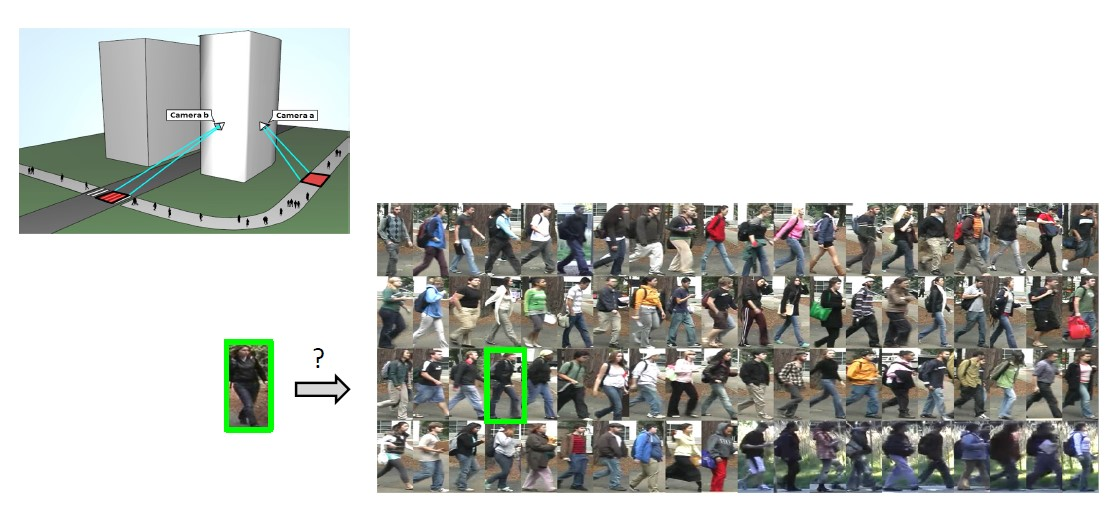
\includegraphics[scale = 1.5]{img/camera1.jpg}
    \label{camera1}
    \caption{Person re-identification}
\end{figure}

Notice that in this case we're not interested in knowing the identity of the person, but just in recognizing him/her over different cameras. Moreover, in modern algorithms we do not consider a single frame, but instead we consider a \textbf{sequence of consecutive frames}, thus both the probe and the gallery are represented by a sequence of overlapping bounding boxes, as showed in \ref{camera2}. In this sense, this approach is \textbf{video-based}.

\begin{figure}[h!]
    \centering
    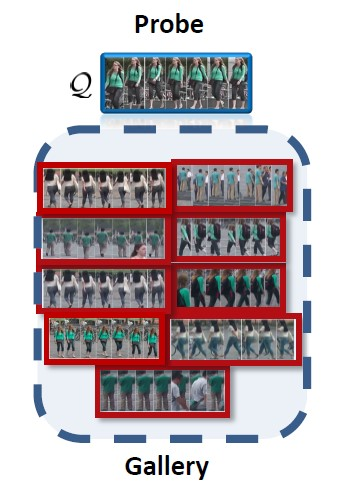
\includegraphics[scale = 1.5]{img/camera2.jpg}
    \label{camera2}
    \caption{Probe and gallery in video-based person re-identification}
\end{figure}

For what concerns the \textbf{solving method} we distinguish:

\begin{itemize}
    \item The \textbf{traditional methods}, which focus on:
    \begin{itemize}
        \item Building a better \textbf{feature representation} of the objects;
        \item Building a better \textbf{distance metric}, i.e. considering a good similarity function, in order to consider both appearance information and motion information;
        \item Ranking the images of the gallery based on the \textbf{pairwise similarity} distances from the query image.
    \end{itemize}
    \item The \textbf{approach of the paper}, which focuses on:
    \begin{itemize}
        \item Using \textbf{standard features} and \textbf{distance metric};
        \item Extracting \textbf{DS's} for each query image;
        \item Performing ranking over \textbf{shortlisted clips}, and NOT over the whole set.
    \end{itemize}
\end{itemize}

In general, the paper takes into account both the \textbf{relationship} between \textbf{query} and elements in the \textbf{gallery} and the relationship between \textbf{elements in the gallery}.

More specifically, the goal of the provided model is to find in the \textbf{gallery DS's of images that contain the query image Q}, i.e. images that are similar to Q and similar to each other (this explains the usage of constrained DS). The pipeline is showed in Picture \ref{camera3}.

\begin{figure}[h!]
    \centering
    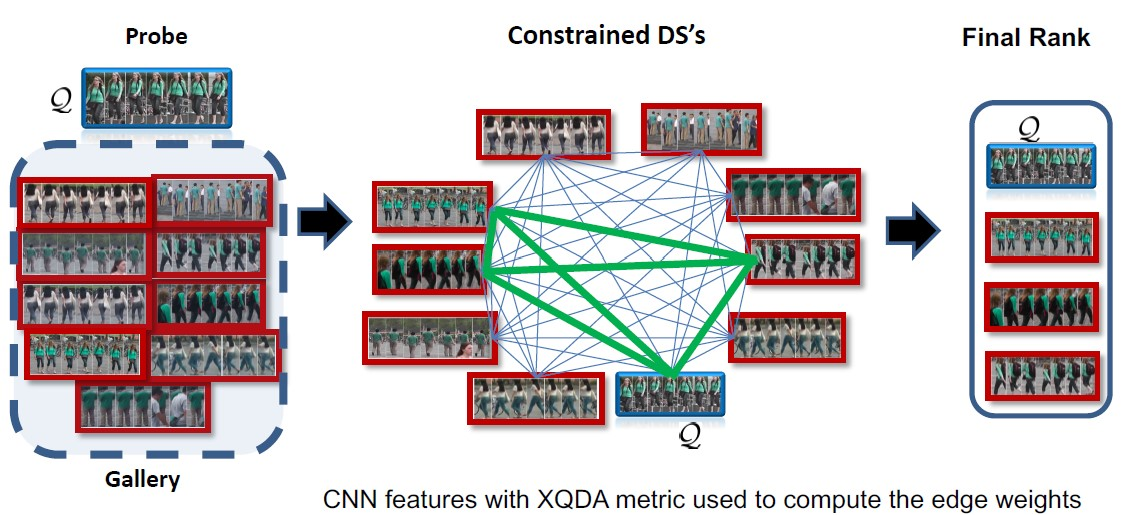
\includegraphics[scale = 1.4]{img/camera3.jpg}
    \label{camera3}
    \caption{Person re-identification with CDS}
\end{figure}

As we can see:

\begin{enumerate}
    \item The gallery images and the probe Q form a \textbf{graph}, where each node represents a \textbf{sequence of frames}, and the \textbf{weighted edges} represent the similarities between frames considering both appearance and motion;
    \item CDS is used for retrieving the \textbf{clusters} of frames similar to Q and to each other;
    \item The frames of the clusters are \textbf{ranked} w.r.t. the similarity with Q.
\end{enumerate}

The model was trained and tested with the largest video re-identification dataset, produced by 6 near-synchronized cameras, and composed of 1,261 identities, 3,248 distractors and tracklets of 25-30 frames long. The qualitative results showed how the model outperformed the existing ones; Picture \ref{camera4} shows the results: the green and red boxes denote the same and different persons with the probes, respectively. Notice that the gallery images are ordered based on their membership score, from the highest to the lowest.

\begin{figure}[h!]
    \centering
    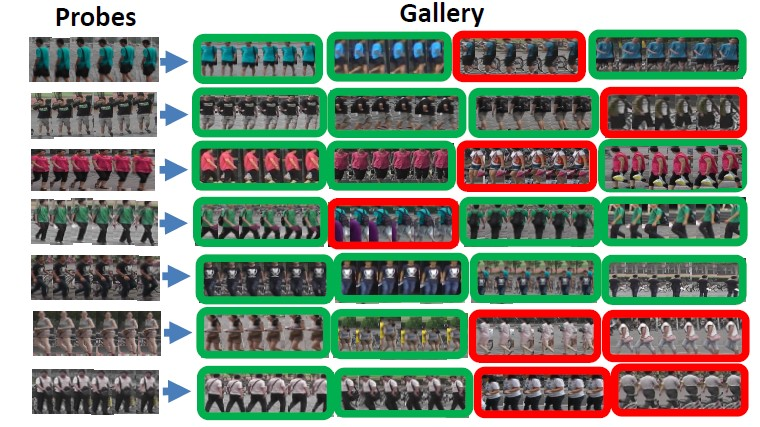
\includegraphics[scale = 1.4]{img/camera4.jpg}
    \label{camera4}
    \caption{Results}
\end{figure}

\subsubsection{Multi-target multi-camera tracking}
We now consider another problem, which is related to the previous one, or rather, the \textbf{multi-target multi-camera tracking problem}. This problem consists on \textbf{tracking multiple objects from multiple non-overlapping cameras}. In this sense, it can be considered a more general version of the previous problem.

\begin{figure}[h!]
    \centering
    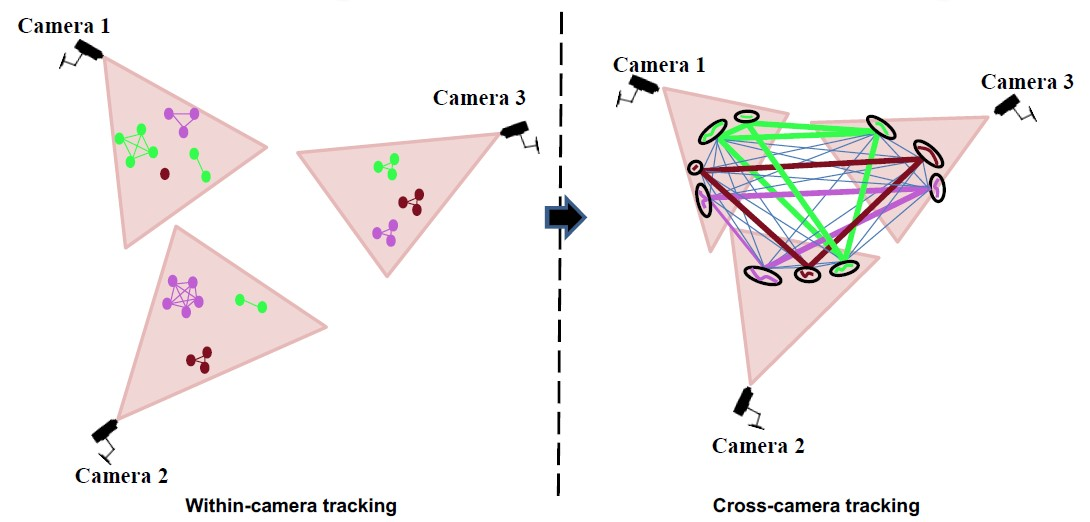
\includegraphics[scale = 1.4]{img/camera5.jpg}
    \label{camera5}
    \caption{Multi-target multi-camera tracking}
\end{figure}

The \textbf{pipeline} of the model that solves the problem is showed in Picture \ref{camera6}.

\begin{figure}[h!]
    \centering
    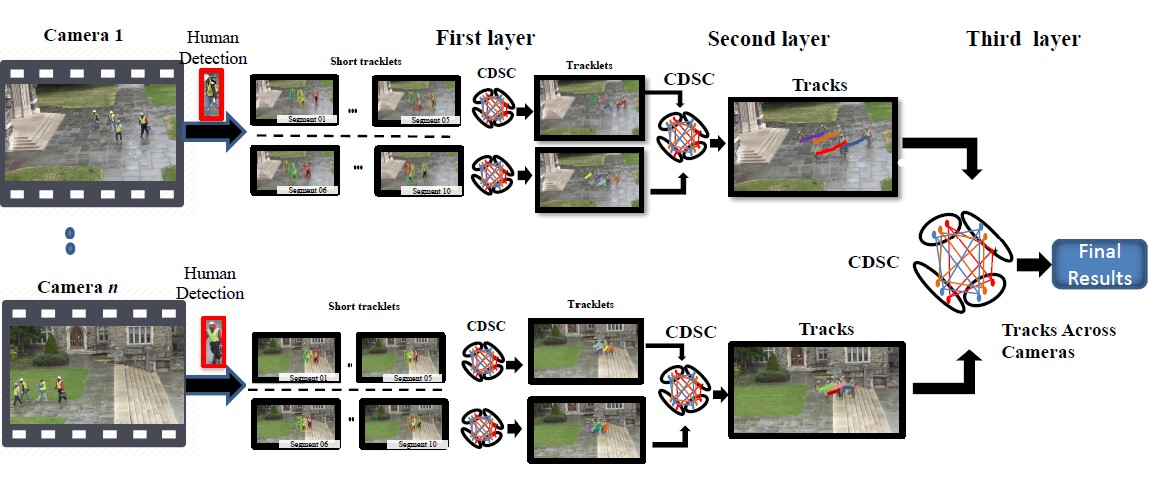
\includegraphics[scale = 1.4]{img/camera6.jpg}
    \label{camera6}
    \caption{Pipeline}
\end{figure}

The steps are the following:

\begin{enumerate}
    \item First of all, an \textbf{human detection algorithm} is executed on the frames of the camera, in order to detect the humans;
    \item First layer: here, the \textbf{short tracklets} obtained by the detection algorithm are represented as a \textbf{graph}. Notice that a short tracklet represents a sequence of consecutive bounding boxes concerning the same person, and all the tracklets compose the nodes of the graph. On the other hand, the \textbf{weights} between the tracklets combine appearance and motion similarity, where:
    \begin{itemize}
        \item \textbf{Appearance similarity} is given by some CNN features;
        \item \textbf{Motion similarity} is given by constant velocity.
    \end{itemize}
    Then, CDS \textbf{clustering} is performed on this graph, obtaining longer tracklets as clusters, as represented in \ref{camera7}.
    
    \begin{figure}[h!]
        \centering
        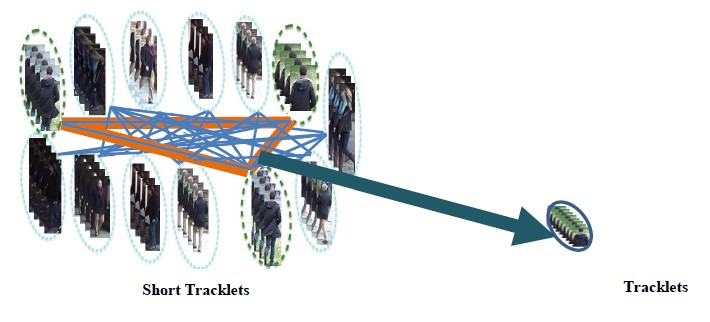
\includegraphics[scale = 1.4]{img/camera7.jpg}
        \label{camera7}
        \caption{Tracklets extraction}
    \end{figure}

    Picture \ref{camera10_13} shows in a more detailed level the execution of the first layer.

    \begin{figure}[h!]
        \centering
        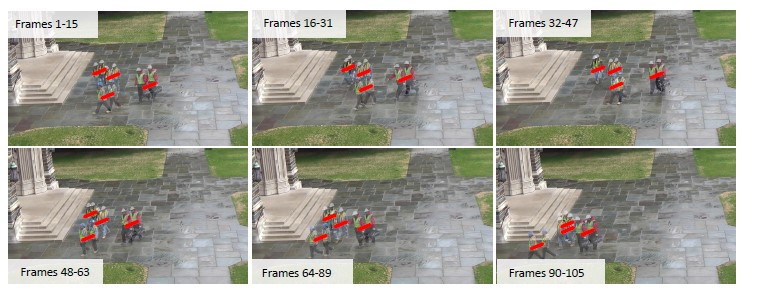
\includegraphics[scale = 1.4]{img/camera10.jpg}
        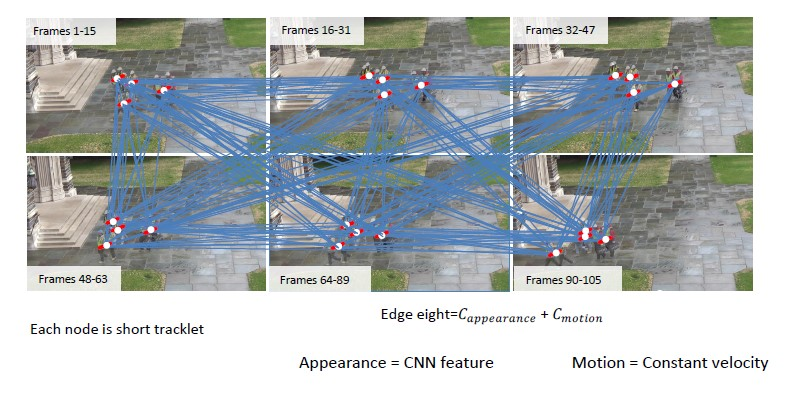
\includegraphics[scale = 1.4]{img/camera11.jpg}
        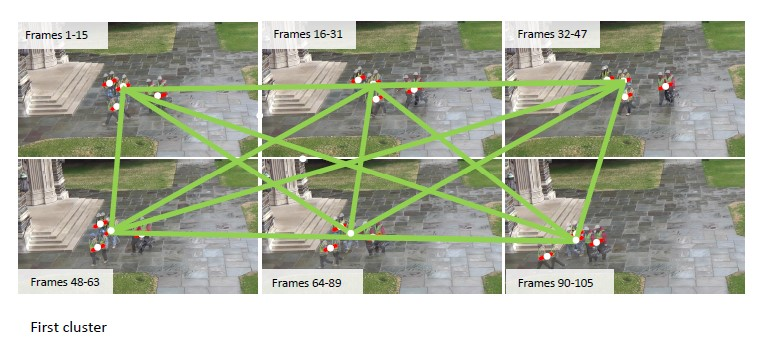
\includegraphics[scale = 1.4]{img/camera12.jpg}
        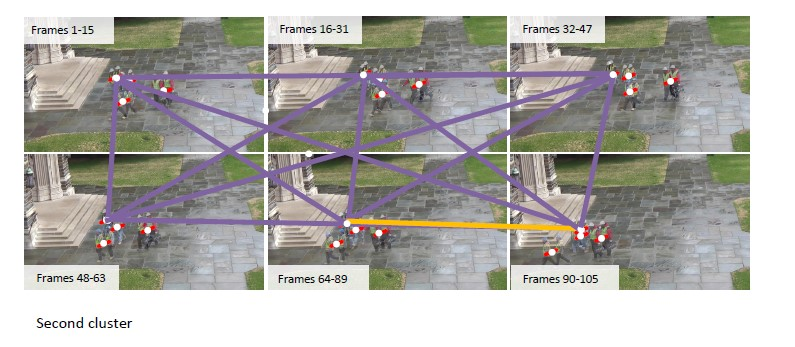
\includegraphics[scale = 1.4]{img/camera13.jpg}
        \label{camera10_13}
        \caption{First layer: detail}
    \end{figure}

    As we can see, the short tracklets form the graph, where the weight of each edge is given by the displayed formula. Then, the DS clusters are displayed.

    \item Second layer: here a new \textbf{graph} is formed, where the nodes are represented by the tracklets returned by the previous phase, and the edges remain the same. Again, CDS \textbf{clustering} is performed, obtaining \textbf{tracks} as clusters, as represented in \ref{camera8}.

    \begin{figure}[h!]
        \centering
        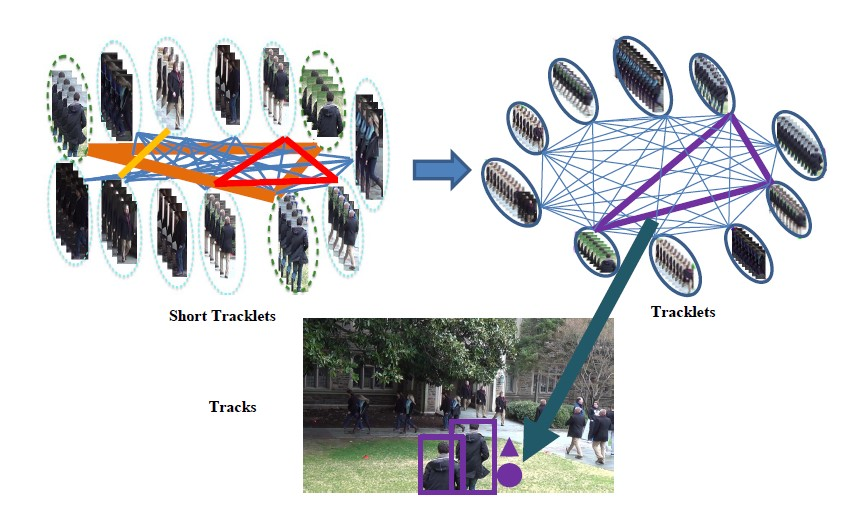
\includegraphics[scale = 1.4]{img/camera8.jpg}
        \label{camera8}
        \caption{Tracks extraction}
    \end{figure}

    \item Third layer: again, a new \textbf{graph} is built using the tracks obtained in the previous layer across all the \textbf{cameras} as nodes, and again a CDS clustering is performed, using the \textbf{cameras} as \textbf{constraints}, as showed in Picture \ref{camera14and15}. 

    \begin{figure}[h!]
        \centering
        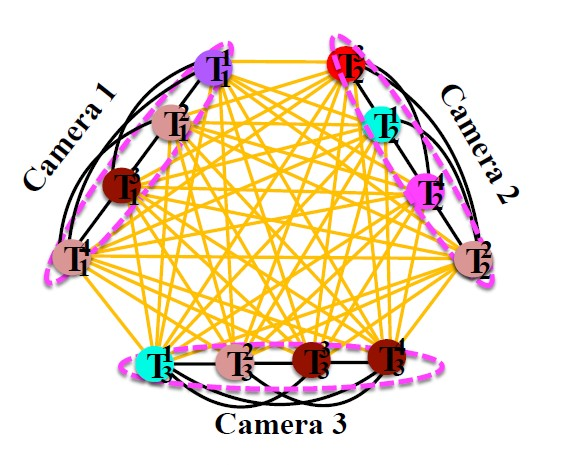
\includegraphics[scale = 1.4]{img/camera14.jpg}
        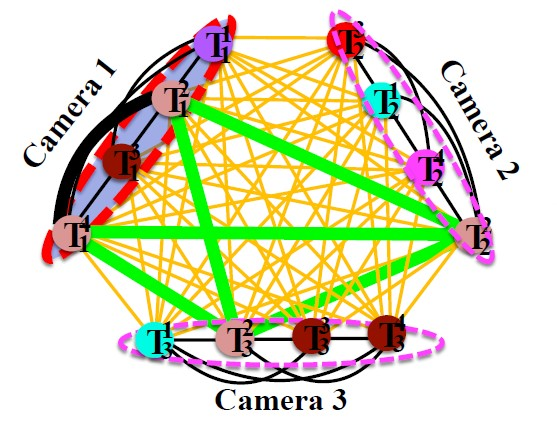
\includegraphics[scale = 1.4]{img/camera15.jpg}
        \label{camera14and15}
        \caption{Third layer}
    \end{figure}
    
\end{enumerate}

Picture \ref{camera9} shows a summary of the functioning and the results of the model.

\begin{figure}[h!]
    \centering
    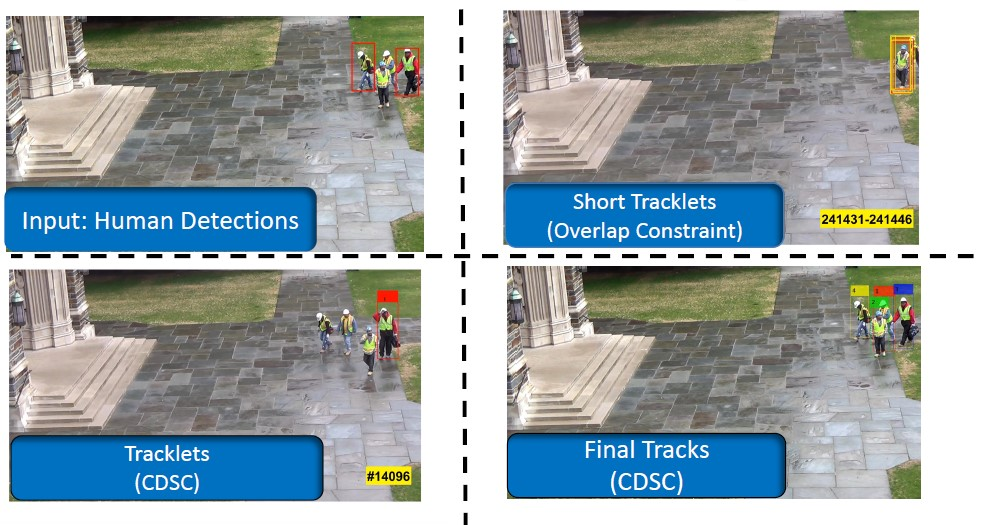
\includegraphics[scale = 1.4]{img/camera9.jpg}
    \label{camera9}
    \caption{Resume}
\end{figure}

The model was trained and tested with the largest MTMC dataset, obtained by 8 fixed synchronized cameras and composed of more than 2 million frames, each containing from 0 to 54 persons, and 2,700 identities. The quantitative results show that:

\begin{itemize}
    \item The fraction of computed detections that are correctly identified (\textbf{IDP}) is \textbf{higher} than the one of two other models;
    \item The fraction of ground-truth detections that are correctly identified (\textbf{IDR}) is \textbf{higher} than the one of two other models;
    \item The ratio of \textbf{correctly identified} detections over the \textbf{average number of ground-truth} and \textbf{computed detections} is \textbf{higher} than the one of two other models;
\end{itemize}

Finally, Picture \ref{camera16} shows the qualitative results obtained by the model.

\begin{figure}[h!]
    \centering
    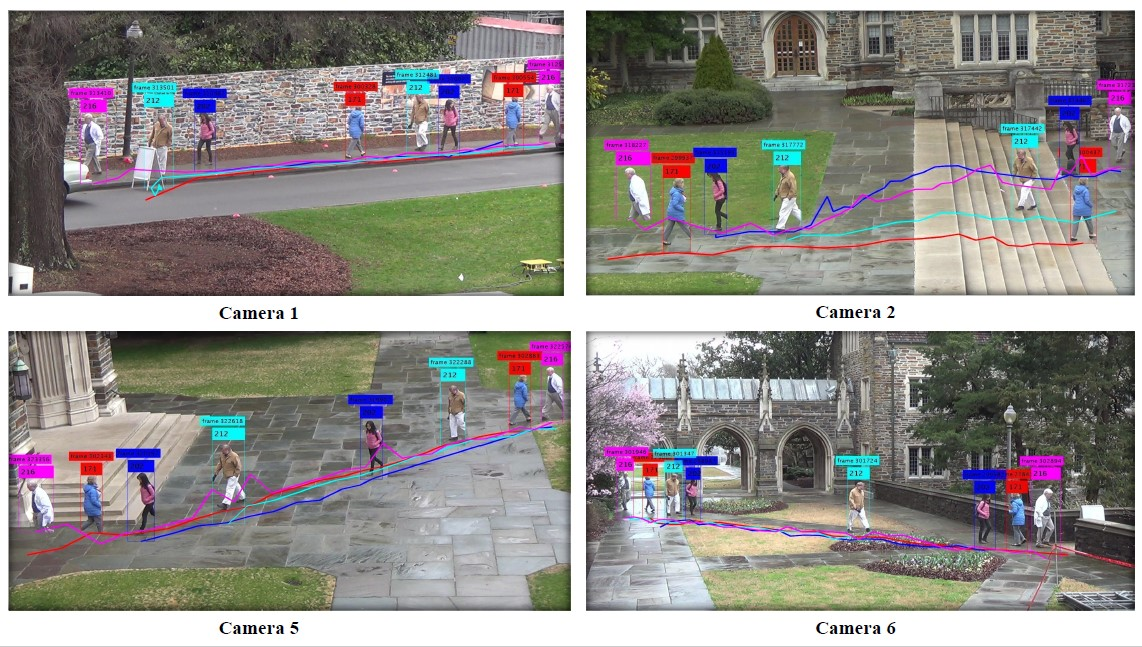
\includegraphics[scale = 1.4]{img/camera16.jpg}
    \label{camera16}
    \caption{Results}
\end{figure}

\subsection{Conclusions}

In conclusion, \textbf{DS} and related concepts shown to be a \textbf{powerful} notion for attacking a variety of \textbf{CV problems}, and ongoing work focuses on \textbf{combining deep learning and DS's for improving performances}.

